\documentclass[twocolumn, 10pt, a4paper]{memoir}

% standard packages
\usepackage{titlesec, blindtext, color}                                  % standard packages
\usepackage[usenames,dvipsnames,svgnames,table]{xcolor} % extra colors 
\usepackage{graphicx}    
\usepackage{amsmath}                                                   % figures
%\usepackage{natbib}                                                          % bibliography
\usepackage{apacite}
\usepackage[english]{babel}
\usepackage{multirow}                                              % correct hyphenation (afbreekstreepjes)
\usepackage{booktabs}                                                     % for midrule in tables
\usepackage{array}
\newcolumntype{P}[1]{>{\raggedright\arraybackslash}p{#1}}
\usepackage[modulo, switch]{lineno}   % use for linenumbers at the sides
% PAGE MARGINS
\usepackage[top=2.5cm, bottom=2.5cm, left=2cm, right=2cm]{geometry}

% FONT
\usepackage[lf]{berenis}
\renewcommand*\familydefault{\sfdefault} 
\usepackage[T1]{fontenc}
% for other fonts, and how to install them, see the LaTeX Font Catalogue:
% http://www.tug.dk/FontCatalogue/

% LINE SPACE
\linespread{1.2}                          % more space between lines
\setlength{\parindent}{7mm}       % indenting first line paragraph
\setlength{\columnsep}{7mm} % space between columns
\linenumbers
% TABLE OF CONTENTS
% for subsubsection headers (e.g. 2.1.3), write subsubsection
% for subsection headers (e.g. 2.1), write subsection
\setsecnumdepth{subsection}        % in text
\settocdepth{subsubsection}              % in table of contents
\renewcommand{\cftdot}{}          % for no dots in table of contents
\cleardoublepage

% HYPHENATION (afbreekstreepjes)
% set words that are not abbreviated correctly (expand list when necessary)
\hyphenation{catch-ment areas a-na-lyse}

\graphicspath{ {./images/} }
%%%%%%%%%%%%%%%%%%%%%%%%%%%%%%%%%
% headers: page numbers and running titles
%%%%%%%%%%%%%%%%%%%%%%%%%%%%%%%%%

\makepagestyle{ruled}
\makeevenfoot{ruled}{}{}{}  % empty footer
\makeoddfoot{ruled}{}{}{}   % empty footer

% header left page (text on left, middle and right slot empty)
\makeevenhead{ruled}{\textcolor{gray}
{\makebox[6mm][l]{\thepage} $|$ \hspace{3mm} \leftmark}}{}{} 

% header right page  (text on right, middle and left slot empty)
\makeoddhead{ruled}{}{}{\textcolor{gray}
{\rightmark \hspace{3mm} $|$ \makebox[6mm][r]{\thepage}}} 

% first page of chapter
\titleformat{\chapter}[hang]{\vspace{-34mm}\huge}{\thechapter\hspace{20pt}\textcolor{gray}{|}\hspace{20pt}}{0pt}{\huge}
\aliaspagestyle{chapter}{chapterheader} % for no page numbers on first chapter page


%%%%%%%%%%%%%%%%%%%%%%%%%%%%%%%%%
% for background figure first page
%%%%%%%%%%%%%%%%%%%%%%%%%%%%%%%%%

\usepackage{eso-pic}
\newcommand\BackgroundPic{%
\put(0,0){%
\parbox[b][\paperheight]{\paperwidth}{\vfill
\centering
\includegraphics[width=\paperwidth,height=\paperheight,keepaspectratio]{figs/backgroundfigure.jpg}%
\vfill
}}}



%%%%%%%%%%%%%%%%%%%%%%%%%%%%%%%%%
%%%%%%%%%%%%%%%%%%%%%%%%%%%%%%%%%
% START
%%%%%%%%%%%%%%%%%%%%%%%%%%%%%%%%%
%%%%%%%%%%%%%%%%%%%%%%%%%%%%%%%%%

\begin{document}

\thispagestyle{empty}                    % otherwise it gives page number on first page
\pagestyle{empty}
\frontmatter
\firmlists                                       % for less space between items in lists


%%%%%%%%%%%%%%%%%%%%%%%%%%%%%%%%%
% TITLE PAGE 
%%%%%%%%%%%%%%%%%%%%%%%%%%%%%%%%%

%\AddToShipoutPicture*{\BackgroundPic} % for backgroundfigure


\twocolumn[
	\begin{@twocolumnfalse}
		\begin{center}
		\vspace*{3cm}
		\fontsize{20}{20} \textbf{Improving rainfall rate estimations with Commercial Microwave Link Signals}\\
		\vspace{2cm}
		\fontsize{20}{20}\textbf{in Sri Lanka using Deep Transfer Learning}\\
		\vspace{9cm}
		\huge \textbf{Ludo Diender}\\
		\vspace{3cm}
		\large \textbf{Supervisors: Hidde Leijnse, Ruben Imhoff and Kirien Whan}\\
		\large \textbf{February 2022}\\
		\vspace{1cm}
		\large \textbf{MSc thesis}
		\large \textbf{Hydrology and Quantitative Water Management Group}\\
		\large \textbf{Wageningen University}\\
		\end{center}
	\end{@twocolumnfalse}]


%%%%%%%%%%%%%%%%%%%%%%%%%%%%%%%%%
% ABSTRACT
%%%%%%%%%%%%%%%%%%%%%%%%%%%%%%%%%

\cleardoublepage

\twocolumn [\begin{@twocolumnfalse}
\chapter*{Abstract}\vspace{-6mm}       % the * prevents numbering of this section
Don't make the abstract too long. See the list of tricks on Blackbord.
\end{@twocolumnfalse}]

%%%%%%%%%%%%%%%%%%%%%%%%%%%%%%%%%
% TABLE OF CONTENTS
%%%%%%%%%%%%%%%%%%%%%%%%%%%%%%%%%

\cleardoublepage
% to remove table of contents name and move the text up
%\renewcommand{\contentsname}{\vspace{-3.5cm}} 
\twocolumn[\begin{@twocolumnfalse}
\renewcommand{\contentsname}{\vspace{-3.5cm}}
\chapter*{Contents}\vspace{-6mm}
\tableofcontents*
\end{@twocolumnfalse}]

  
%%%%%%%%%%%%%%%%%%%%%%%%%%%%%%%%%
% INTRODUCTION
%%%%%%%%%%%%%%%%%%%%%%%%%%%%%%%%%

% start on right side of page
\cleardoublepage 

% start with page numbering 1, 2, 3 instead of i, ii, iii
\pagestyle{ruled}
\mainmatter          

% Chapter name
\chapter{Introduction}\vspace{-6mm} 
\section{Context and motivation}

Having ample and correct precipitation data is important for a plethora of applications, including flood warnings, agriculture, river safety and shipping routes \shortcite{Chwala2019}. In urban areas, an even higher spatial and temporal resolution of rainfall is needed, due to the complex and quickly responding urban hydrological system \shortcite{Overeem2011}. A high rain gauge density can help in providing this resolution in urban areas \shortcite{Yoon2017}, but is not always availabe. Commercial Microwave Links (CML) do typically have a high density in populated areas and could therefore help in retrieving these high-resolution urban precipitation data. CML are back-haul links used by telecommunication companies to transfer information from one telecom station to the next using microwave signals. The links' signals get attenuated by rainfall by means of scattering and absorption. The received signal level is measured and stored by the telecommunication companies for monitoring purposes and can be used to retrieve path-averaged rainfall rates by calculating the attenuation. In the past 25 years, CML have been recognized as a valuable opportunistic method to measure rainfall \shortcite{Leijnse2007, Ruf1996}. Especially in data-scarce areas, where little precipitation is measured, CML have proven to be an excellent additional information source for precipitation data \shortcite{Overeem2021,Doumounia2014,Diba2021}.   

The first studies on the use of CML signals to retrieve rainfall rates were done by using a specific Power Law (PL) to relate the attenuation of the signal and the rainfall rate \shortcite{Overeem2011,Leijnse2007}. This method, which includes a wet-dry classification, baseline estimation, wet antenna attenuation estimation and finally a rainfall rate retrieval, has yielded good results in multiple studies \shortcite{deVos2019,Graf2020,Fencl2017}. Recently, the community has been exploring a more data-driven approach in the form of neural networks of different architectures. Neural networks are a subpart of Machine Learning that is inspired by the neural structure of the brain. A neural network consists of different layers of nodes (neurons) that are connected to each other. If the network contains more than one layer, it is considered a deep network and Deep Learning is used as equivalent naming. A neural network is able to learn the relationship between the input and output, without intervention from a researcher. Studies have been performed in Sweden, Israel \shortcite{Habi2019}, Germany \shortcite{Polz2020}, South Korea and Ethiopia \cite{Diba2021} on the use of such data-driven networks in relating CML signals to rainfall rates. Previous studies have shown that data-driven models can be more accurate, less time-demanding and more robust in estimating rainfall rates compared to the PL method \shortcite{Polz2020,Pudashine2020}. Neural networks are not a novelty in predicting rainfall \shortcite{French1992}, but the application to CML data has recently gained popularity.

\begin{figure}[t]
	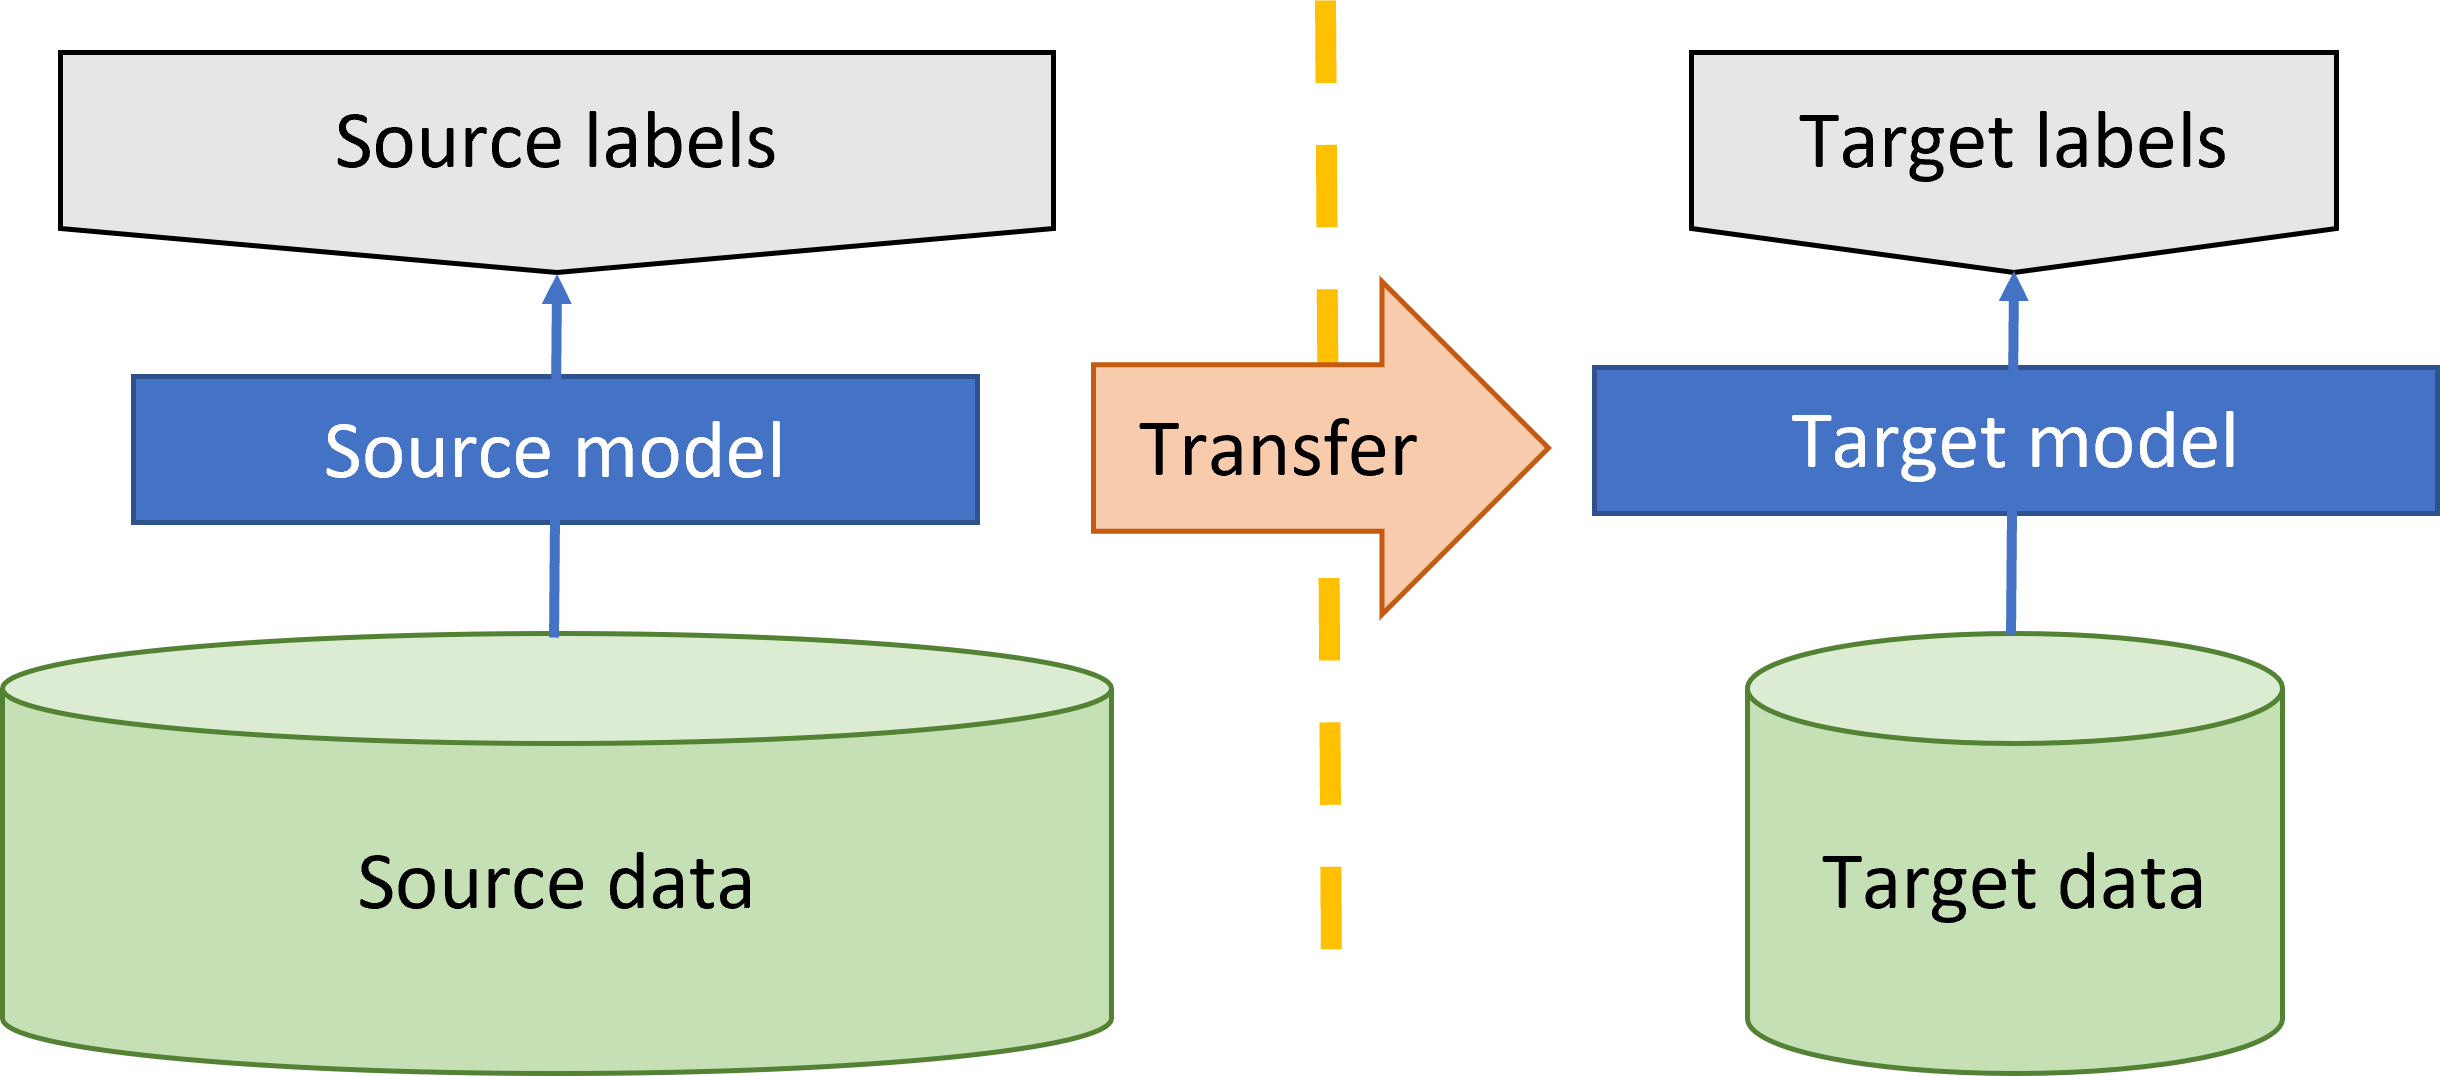
\includegraphics[width=8cm]{Transfer_learning_concept}
	\caption{Concept of transfer learning. Adapted from \protect\cite{Sarkar2018} }
	\label{fig:transferconcept}
\end{figure} 

One of the disadvantages of using data-driven methods like neural networks, is the dependency on a large training data set. Neural networks need this large dataset to learn the relationships between input and output. In areas with less or little available training data, which is generally the case in less developed countries, transfer learning provides the opportunity to adapt an already existing model with a certain structure to do a slightly different task \cite{TanYear}. The concept of transfer learning is based on the way humans learn. When humans learn a new task, we do not start from scratch. We use previous knowledge and skills to quickly adapt to the new task. When learning to ride a motorcycle, it helps if you already know how to ride a bike. Concepts like balance and steering can be transferred from the latter task to the former, thus speeding up the learning process. 
The technique exploits the availability of data in the source domain and is able to transfer that knowledge to the target domain. It does so by relaxing the underlying assumption that training and test data for a Machine Learning model should be independent and identically distributed \cite{Weiss2016}. Training data from a different domain might not fulfill this assumption but it can still carry important information about the modelled concept. A conceptual picture of transfer learning can be seen in figure \ref{fig:transferconcept}. Although used quite often in different applications \cite{Zhuang2021}, transfer learning concerning environmental sciences has so far primarily been applied in wind farm modelling \shortcite{Hu2016,Qureshi2017}. The potential of transfer learning in CML rainfall estimations has not been studied before. 

Recent research focused on the use of CML data to measure rainfall in tropical regions, more specifically Sri Lanka \shortcite{Overeem2021} and Brazil \shortcite{RiosGaona2017a}. The relatively small amount of reference rain gauges in Sri Lanka especially made this research more challenging compared to well-equipped countries like the Netherlands \shortcite{Overeem2013}. Both of the two studies mentioned above (Sri Lanka and the Netherlands) are based on the PL method. There have not been any efforts yet to analyze the potential of CML for rainfall retrieval using data-driven methods for neither the Netherlands nor Sri Lanka. This research aims to fill this knowledge gap by creating a neural network used for CML rainfall retrieval in the Netherlands and by studying the potential of transer learning within the Dutch context.

\section{Research questions}
This study focusses on two main research questions.
1) How does a Neural Network perform on estimating rainfall rates from Dutch Commercial Microwave Link data?
2) How can the concept of transfer learning be applied to enhance performance or modelling efforts?
By answering these questions, this study will give a first impression of the potential of Deep Transfer Learning related to precipitation estimation with CML. 


\section{Thesis contents}
This thesis starts with a description of the data that is used (Section~\ref{ch: field}). In Section~\ref{ch: methods} the methodology of this study is described. This includes an explanation on Neural Networks, data preprocessing, transfer learning and the set-up of this model study. Afterwards, in Section~\ref{ch: results} the results are presented. These results and the approach used in this study are discussed in Section~\ref{ch: discussion}, which is followed by the conclusion in Section~\ref{ch: conclusion}.






%%%%%%%%%%%%
% FIELD SITE AND DATA
%%%%%%%%%%%%

\cleardoublepage
\chapter{Field site and data}\vspace{-6mm} 
\label{ch: field}
Some text here about how the field site and data are structured?

\section{Commercial Microwave Link data}
	\subsection{Netherlands}
		\paragraph{Location of the links}
		First paragraph 
		text text text text text text text text text text text text text text text text text text text text text
		\paragraph{Static vs dynamic data}
		First paragraph 
		text text text text text text text text text text text text text text text text text text text text text
		\paragraph{Freq,temp res and timespan}
		First paragraph 
		text text text text text text text text text text text text text text text text text text text text text
	\subsection{Sri Lanka}
		\paragraph{Location of the links}
		First paragraph 
		text text text text text text text text text text text text text text text text text text text text text
		\paragraph{Static vs dynamic data}
		First paragraph 
		text text text text text text text text text text text text text text text text text text text text text
		\paragraph{Freq,temp res and timespan}
		First paragraph 
		text text text text text text text text text text text text text text text text text text text text text

\section{Reference precipitation data}
	\subsection{Netherlands}
		\paragraph{Obtained from (provider)}
		First paragraph 
		text text text text text text text text text text text text text text text text text text text text text
		\paragraph{Temporal and spatial resolution}
		First paragraph 
		text text text text text text text text text text text text text text text text text text text text text
		\paragraph{Quality and availability}
		First paragraph 
		text text text text text text text text text text text text text text text text text text text text text
	\subsection{Sri Lanka}
		\paragraph{Obtained from (provider)}
		First paragraph 
		text text text text text text text text text text text text text text text text text text text text text
		\paragraph{Temporal and spatial resolution}
		First paragraph 
		text text text text text text text text text text text text text text text text text text text text text
		\paragraph{Quality and availability}
		First paragraph 
		text text text text text text text text text text text text text text text text text text text text text



%
%
%text text text text text text text text text text text text text text text text text text text text text
%text text text text text text text text text text text text text text text text text text text text text
%text text text text text text text text text text text text text text text text text text text text text
%text text text text text text text text text text text text text text text text text text text text text
%text text text text text text text text text text text text text text text text text text text text text
%
%\section{Figures}
%
%Figures are moved automatically to nice places.
%
%\begin{figure}[t]
%\center
%\includegraphics[width=\columnwidth]{figs/ponds.jpg}
%\caption{Single column figure, located in the directory of the field sites chapter}
%\label{fig: ponds}
%\end{figure}
%
%\begin{figure*}[t]
%\center
%\includegraphics[width=2\columnwidth]{C:/Users/ludod/Documents/MSc Thesis/LaTeX thesis template/figs/ponds}
%\caption{Two-column figure located somewhere else on my hard drive.}
%\label{fig: GWD world}
%\end{figure*}
%
%
%
%
%
%text text text text text text text text text text text text text text text text text text text text text
%text text text text text text text text text text text text text text text text text text text text text
%text text text text text text text text text text text text text text text text text text text text text
%text text text text text text text text text text text text text text text text text text text text text
%text text text text text text text text text text text text text text text text text text text text text
%
%
%
%\section{Tables}
%
%Tables are moved automatically to nice places too.
%
%\begin{table}[t]
%\caption{Parameter values obtained by optimization with HydroPSO using different objective functions.}
%\label{tab: testtable}
%\centering
%\begin{tabular}{lllll}
%\toprule
%fit on:&$Q^2$&$Q$&$\sqrt{Q}$&$d_\mathrm{G}$\\
%\midrule
%$c_\mathrm{W}$&400&380&379&107\\
%$c_\mathrm{V}$&1.8&0.8&8.2&0.2\\
%$c_\mathrm{G}$&5.3&5.0&5.0&5.0\\
%$c_\mathrm{Q}$&1&4&12&87\\
%\bottomrule
%\end{tabular}
%\end{table} 
%
%\subsection{Equations}
%
%\begin{equation}
%Q = \overline{v} \times A
%\end{equation}
%\label{eq: testequation}
%
%\section{References and citations}
%\label{sec: header 2}
%
%
%\subsection{References}
%
%
%Refer to Chapter~\ref{ch: field}.
%
%Refer to Section~\ref{sec: header 2}.
%
%Refer to Figure~\ref{fig: GWD world}.
%
%Refer to Table~\ref{tab: testtable}.
%
%Refer to Equation~\ref{eq: testequation}.
%
%
%\subsection{Citations}
%
%
%Floods are important \citep{Brauer2011}.
%
%\cite{Brauer2011} state that floods are important.
%
%Floods are important \citep[according to][]{Brauer2011}.
%
%\section{Section header 3}
%
%\subsection{Subsection header}
%
%\subsubsection{Subsubsection header}



%%%%%%
% METHODS
%%%%%%

\chapter{Methods} \label{ch: methods}
This chapter describes the methodology of this study. The chapter starts with a general explanation on Neural Networks and their functioning, to get acquainted with terms and parameters in Section \ref{NN explain}. Section~\ref{datapreprocess} deals with the preprocessing of the input data to the model and subsequently model selection is described in Section~\ref{modelselection}. The combination of Neural Networks and the input data in this study is discussed in Section (>>>>). Section~\ref{EvalStats} is concerned with the validation of the model results and performance of the model related to the benchmark method RAINLINK. The final part of this chapter deals with transfer learning and how this is applied in this study (Section~\ref{transferlearning})
	\section{Neural network explanation} \label{NN explain}
		\subsection{Goal and concepts of neural networks} \label{NNConcepts}
		Neural networks are a subset of models within the Machine Learning (ML) environment. All models within the ML space are data-driven, i.e. without pre-specified relationships between input and output. These data-driven models aim to figure out this relationship via self-learning techniques. 
		The biggest advantages of such models are that 1) they are very versatile: they can adapt to various circumstances and can be used in a wide range of applications, and 2) they can learn relationships that we do not have a physical explanation for yet. Through multiple iterations, the models can improve by minimizing or maximizing a loss function. The loss function can be interpreted as a score for the model: the worse the score, the more the model needs to adjust itself (see Section~\ref{Learning NN}).It improves by optimizing parameters of differential equations in the model. Similar to physically-based models, it is up to the modeler to determine when the model performs well enough. The self-learning ML models will stop learning after a certain criterion is met, or when a specified number of iterations has passed. 
		
		Neural networks are inspired by the structure of the human brain with neurons and synapses, hence the name Neural network. The network consists of one or multiple layers of nodes that are connected with each other. When the network has more than one layer, it is called a Deep Neural Network and it is referred to as Deep Learning. Every single connection between nodes (or between nodes and input/output) is represented by a weight and a bias. These weights and biases are the bread and butter of neural networks. They determine the underlying relationships between different parts of the input signal, the connections within the model and the relation to the final output. Training a neural network is all about adjusting the weights and biases in such a way that the desired output is created. At every node, a weighted sum is calculated based on these weights and biases and it is passed to an activation function. This activation function yields one value, which will be passed to the following nodes in the model. 
		Because of the very general structure of neural networks, they form a very versatile set of models. Research efforts in neural networks span from image classification and speech recognition to time series prediction and weather forecasts. 
		
		\subsection{Neural network architectures} \label{NN architecture}
		The versatility of neural networks allows for a wide range of different model architectures to choose from. Every architecture has its own strengths and weaknesses. For image recognition for example, the most common type of neural network is a Convolutional Neural Network (CNN). In time series prediction, the most common architecture is the Recurrent Neural Network (RNN), which is therefore most suited for precipitation estimation using Commercial Microwave Links.
		
		RNNs are looping-based architectures, which make them ideal for dealing with sequences. The core unit of RNNs, the Recurrent Unit (the lightgreen blocks in Figure \ref{fig: multilayer RNN}), is used multiple times. The output of the unit is added to the input of the next step in the same recurrent unit. This creates an architecture that is well suited for time series with sequential data patterns. How many layers of these recurrent units are used in a model depends on the modeler and can be tuned (see Section \ref{modelselection})
		
		One of the limitations of default RNNs is the lack of memory in the model. While information within a sequence is passed through the model well, information from previous sequences is lost. A Long Short Term Memory (LSTM) model circumvents this problem by having an extra stream of information through the model. This stream of information carries aspects of the previous sequences and can therefore be considered a memory. In an LSTM, more information of the former step is taken into account when making a
		prediction for the current step. This creates a memory in the model, where information from a longer time ago can still be valuable in the current prediction. Similar to \cite{Habi2019}, this study uses a LSTM neural network. A many-to-one architecture is used, which means that a sequence of signal levels is used to predict one rainfall rate at a specific timestep. 
		
		\begin{figure} 
			\center
			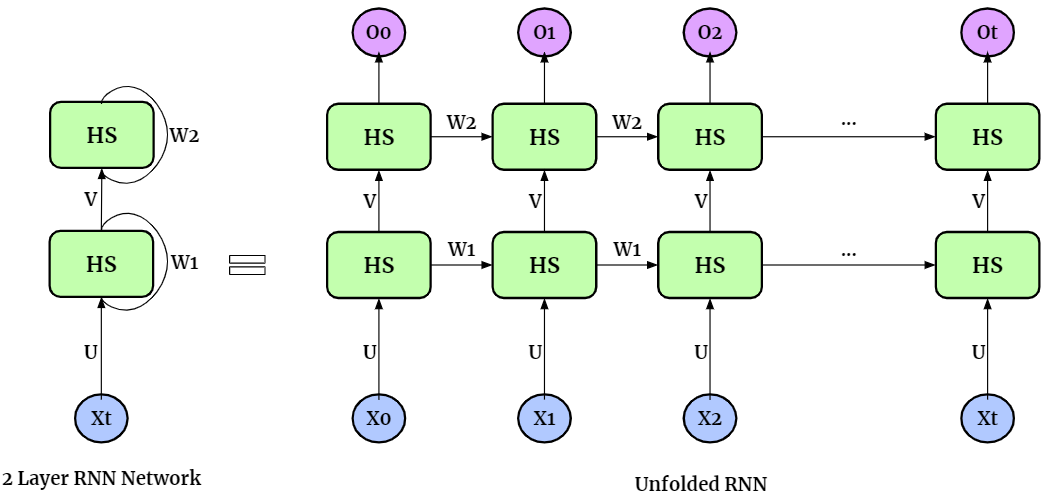
\includegraphics[width=\columnwidth]{C:/Users/ludod/Documents/GitHub/Thesis_HWM2021/Thesis/multilayer_RNN.png}
			\caption{\textit{Schematic representation of a two-layer unfolded RNN. HS represents the hidden state,X is the input, O is the output and U, V and W are weight and bias vectors associated with the model}}
			\label{fig: multilayer RNN}
		\end{figure}
		
		\subsection{Learning process of neural networks} \label{Learning NN}
		The self-learning ability of Neural Networks is mainly relying on the loss function. The model calculates the error between its output and the target output and tries to adjust accordingly. The selected loss function determines amongst others the behavior of the model. In this study, a standard Mean Square Error (MSE) loss function is used as a basis (see Eq.~\ref{eq: MSE}). 
		\begin{equation} \label{eq: MSE}
			MSE = \frac{1}{n} \sum_{i=1}^{n} (y_i - \hat{y})^2
		\end{equation}
		where ${y_i}$ is the predicted 15-min interval precipitation and $\hat{y}$ is the observed 15-min interval precipitation.
		MSE as a loss function has been used before in similar studies \cite{Pudashine2020, Diba2021}. These studies, however, had a more elaborate preprocessing of the data to correct for the inherently skewed nature of precipitation distributions. \citeA{Habi2019} showed that the loss function can also be altered to correct for this skewedness by using a Rain Distribution Factor (RDF). In this research, the application of a RDF serves two purposes:
		
		\begin{itemize}
			\item Penalize negative predictions more to force the model into predictions bigger than or equal to zero. A random initialization can cause negative output which is physically impossible.
			\item Penalize the model more for higher target variables. This steers the model towards a better prediction of the actual precipitation events. 
		\end{itemize} 
	
		The RDF is defined in Eq~\ref{eq: RDF},
		
		\begin{equation} 
			\label{eq: RDF}
			RDF=\begin{cases}
				3, & y_i < 0\\
				1-y_s e^{y_r\cdot{}\hat{y}}, & \text{otherwise}.
			\end{cases}
		\end{equation}	
		where $y_i$ is the predicted rainfall rate, $\hat{y}$ is the observed rainfall rate and $y_s$ and $y_r$ are hyperparameters, set to $0.95$ and $-5$ respectively in accordance with \citeA{Habi2019}.
		
		The combination of Eq~\ref{eq: MSE} and Eq~\ref{eq: RDF} leads to the final loss function used in this thesis (Eq~\ref{eq: final_loss})
		
		\begin{equation}
			\label{eq: final_loss}
			Loss = \frac{1}{n} \sum_{i=1}^{n} RDF \ (y_i - \hat{y})^2 
		\end{equation}
	
		To update and improve the model prediction, a propagation algorithm is selected. Such a propagation algorithm is a mathematical set of equations that determines how the model learns. In this study, Stochastic Gradient Descent (SGD) will be used. SGD is one of the most commonly used algorithms to improve neural networks. SGD is based on a gradient descent algorithm to optimize the loss function In simple terms: the method is looking for an optimum (minimum or maximum) per weight. Based on this gradient, the weight is adjusted up or down to minimize the loss function (MSE in this study). As calculating the full gradient field for all weights present in the model is a tedious task, SGD takes a randomly selected subset of the data and uses that to calculate the gradients. This might lead to more steps, but the steps are less computationally intensive and typically lead to an improved performance.  
		The SGD method is back-propagated. This implies that the final layer of the network is updated first and the learning process works itself back to the start of the model. In this study, the fully connected layer at the end of the RNN is updated first before the model improves and adjusts in the recurrent unit itself. A back-propagated model is chosen in this study since it is the most common type of neural network, easy to implement, fast, flexible and generally good. 
		 
		\subsection{Available hyperparameters} \label{Avail hyper}
		The versatility of Neural Networks is generally perceived as one of the biggest advantages of these type of models. However, it does leave the modeller with a lot of options to choose from in creating a Neural Network for their specific task. The parameters that refer to the architecture and set-up of the Neural Network are called hyperparameters. Table~\ref{tab: hyperparamtable} highlights the available hyperparameters in this model. The hyperparameters can be divided in three groups: Structure, Data and Effiency. Structure hyperparameters relate to the structure of the model: how is it designed and how often will it run. Data parameters are related to the input data into the model; the type of data and the goal with the data determine these hyperparameters. The Efficiency group entails hyperparameters that relate to the time it takes the model to run. In this group, there's always a balance between performance and computational intensity.
		\begin{table*}[ht]
			\caption{Available hyperparameters in this study.}
			\hspace*{\fill}
			\label{tab: hyperparamtable}
			\centering
			\renewcommand{\arraystretch}{1.5}
			\begin{tabular}{P{0.8cm}P{2.0cm}P{12.8cm}}
				\hline
				Group&Hyperparameter&Description\\
				\hline
				\multirow{4}{*}[-38pt]{\rotatebox{90}{Structure}}&Hidden size&Size of the intermediate hidden output. Higher hidden size allows for more complex relations\\
				&Learning rate&A multiplication factor that influences the speed at which the weights in the model are updated with each SGD step. A high learning rate makes the model learn faster, but also makes it more prone to overfitting.\\
				&Number of epochs&The number of iterations the model performs to reach the final prediction. More epochs improve the performance of the model but take sginificantly longer to run.\\
				&Number of layers&Total number of layers in the model. A higher number of layers creates a model that can better identify complex dependencies in the data.\\
				\midrule
				\multirow{2}{*}[-10pt]{\rotatebox{90}{Data}}&Sequence length&Length of datasample used to predict one target value.\\
				&Loss function&Metric that is used to judge the model performance on. Can be tailored towards the goal of the model.\\
				\midrule
				\multirow{4}{*}[-20pt]{\rotatebox{90}{Efficiency}}&Activation function&Function within each node that determines the value of the node as a consequence of the weighted average\\
				&Batch size&The size of each batch of data that is fed to the model. The larger the batch size, the faster the model will be able to learn, but the less possiblities it has to update its weights and biases.\\
				&Learning algorithm&The algorithm that is used to update the weights and biases of the model internally.\\
				&Scheduler&The algorithm that is used to run multiple combinations of hyperparameters simultaneously and decides when to quit with some of the runs\\
				
				\bottomrule
				
			\end{tabular}
			\hspace*{\fill}
		\end{table*}
		
		The process of calibrating hyperparameters in order to find an optimal combination (if it exists) is refered to as tuning. Not all hyperparameters were automatically tuned. Only the Structure hyperparameters were tuned, as the other two hyperparameter groups need to be determined based on the input data and the available computational resources. More details on the automatically tuned Structure hyperparameters can be found in Section \ref{RayTune}. The Data and Efficiency group of hyperparameters are set based on convenience and literature study and will be elaborated on in Section \ref{Nonauto tuning}.
		
	\section{Data preprocessing} \label{datapreprocess}
		\subsection{Connecting CML and reference data}
		To train the Neural Network, a feature set and a target set is needed. For every link in the CML dataset, the corresponding amount of precipitation has been determined. To obtain this value, the middle point of each link has been determined and connected to the corresponding radar cell. This midpoint method is commonly used in CML research (refs). More elaborate methods have been used by \shortciteA{Leijnse2007} for example, where a weighted sum of all cells that the link passes through was created. The impact of this decision will be discussed further on in this thesis. 
		\subsection{Error filtering}
		A large part of the RAINLINK algorithm consists of error filtering. Because the algorithm cannot distinguish a signal distortion by rain or by a bird, this filtering is necessary. The spirit of Deep Learning models is that these errors don't need to be filtered out manually. Similar to Habi et al., just the 'no data' values have been removed from the dataset. The model is expected to handle other noise in the data by learning the patterns and adjust accordingly.
		\subsection{Data splitting and scaling}
		A Deep Learning model with a varying set of hyperparameters needs three independent datasets to run. The training dataset is used to improve the models weights and parameters and is fed through the SGD algorithm, in which the model is updated in a backwards propagating fashion. The testing dataset is subsequently used to independently judge the capabilities of the model. After training, this set is used to calculate an error metric to see how well the model is doing. This error metric (MSE in this study) is used to update the weights in the model. An independent dataset is needed to prevent overfitting of the model, a very common problem in Machine Learning models. 
		As different models with different combinations of hyperparameters are tested, a third independent dataset is needed to check how well the best model out of this sample set performs. Again, the main goal is to prevent overfitting. 
		
		In creating the three separate datasets, multiple approaches can be taken. The core of the split is based on the IID principle (Independent and Identically Distributed):
		
		\begin{itemize}
			\item There is little to no information leaked from one set to the other (truly independent datasets)
			\item There is enough data in each of the sets to cover a wide range of events and situations (comparable datasets and thus assumed identically distributed)
		\end{itemize}
		The data for the Netherlands has been split in a 40/40/20 way of training, testing and validating respectively. Previous studies use varying ratios in splitting the data, with the one common aspect being a smaller validation set compared to the trainig and testing \cite{Polz2020,Diba2021,Pudashine2020}.
		The year 2011 is used for training, 2012 for testing and 2013 (up until July 21st) for validating. By taking full years for training and testing, all seasons are incorporated and the datasets are assumed to be closer to being identically distributed. NOTE ABOUT 2011, WHICH HAD A VERY VERY DRY SPRING.
		There is a tradeoff in the IID assumption that created the split as decided upon in this study. Because of the dry spring, the years 2011 and 2012 are not identical. However, wherever the two datasets meet in time, there is a chance of information leaking from one dataset to the other. Therefore, this split by full years was still prefered. For the validation set, half a year is taken due to limitations in data availability. As the validation set is only used to judge the final model, and not to update the model anymore, this dataset can be smaller as in (LITERATURE). 
		
		Having large outliers and ranges in the input data can cause the SGD algorithm to have exploding gradients. Therefore, a scaling has been applied to the features and targets. Similar to \cite{Kilmartin1972}, the precipitation data were log-transformed. Afterwards, they were scaled with the minimum and maximum per dataset, to create a value between 0 and 1. A similar scaling has been applied to the features (RSL), as they are scaled to their min and max value. 
		The different datasets are scaled differently. They all fit between 0 and 1, which is convenient for the SGD algorithm. If all datasets were scaled in the exact same way, it would inevitably lead to data leakage from one dataset to the other, violating the IID assumption as discussed before. 
		

	\section{Model selection} \label{modelselection}
		\subsection{Automated hyperparameter tuning} \label{RayTune}
		A full grid search on all hyperparameters available to find the best combination is computationally infeasible. Therefore, this study uses 25 random combinations of hyperparameters, all within a limited range of values. This number of combinations is chosen to have a trade-off between computational intensity and having ample combinations to ensure a decent search.
		Selecting the combinations is done using the RayTune package, which is a tuning-specific Python package that interacts with PyTorch (used in this study) and other Deep Learning packages. This study uses the Async Successive Halving Algorithm Scheduler (ASHA) to effectively search the hyperparameter space. The ASHA Scheduler is able to effectively implement parallelism (to decrease runtime) and a hard early stopping mechanism to terminate runs if they are not amongst the best few models after a while \cite{Li2018}. The ASHA Scheduler is the most common scheduler available in RayTune and performs well in most cases when no specific instructions regarding hyperparameter tuning are needed.  
		The random combinations allow for quickly identifying the most sensitive hyperparameter and tune it specifically if needed. The best combination of hyperparameters is used to calculate the model performance based on the final independent validation dataset. The ranges for the calibrated hyperparameters can be found in Table~\ref{tab: raytunetable}
		
		\begin{table}
			\caption{Ranges for the automatically tuned hyperparameters using RayTune.}
			\label{tab: raytunetable}
			\centering
			\renewcommand{\arraystretch}{1.5}
			\begin{tabular}{p{2.5cm}p{4.2cm}}
				\hline
				$Hyperparameter$&$Range$\\
				\hline
				Hidden size&$[64,128,256]$\\
				Learning rate&$1e^{-6} - 1e^{-3}$\\	
				Number of epochs&$(1 - 20)$\\
				Number of layers&$[2,4,8,16]$\\
				\hline
			\end{tabular}
		\end{table}
		
		\subsection{Non-automated hyperparameter tuning} \label{Nonauto tuning}
		\textbf{Hyperparameters that are related to the data rather than the model itself are not tuned automatically.} Hyperparameters in the Data group are tuned, but in a slightly less rigid way as it is easier to deduct which values should perform well on the input data.
		The sequence length is partly determined by how long rainfall events typically last in the Netherlands and their autocorrelation. As a starting value, a sequence length of 4 (15-min) timesteps is used. This means that the past hour is used to predict the rainfall rate at the current time step. Other larger sequence lengths will be explored to see whether this improves the performance of the model. (SIDENOTE FOR THESISRING: number still needs to be explored)
		The loss function has a direct relation to the distribution of the input data. As precipitation data is not normally distributed, a standard MSE loss function might put more emphasis on keeping the prediction lower and therefore missing out on large precipitation events. However, a slightly different adjusted loss function is used as well (STILL SEE WHICH ONE MIGHT BE USEFUL) to see if that improves the results on the independent validation set. 
	\section{Evaluation metrics and summary statistics} \label{EvalStats}
	\section{Transfer learning} \label{transferlearning}
	The act of Transfer learning relies on using a pretrained model for a different task. In this study, the pretrained model on the Netherlands will be used to estimate rainfall rates in Sri Lanka. Transfer learning of RNN models can be done in two different ways, which will shortly be discussed in the following sections.
		\subsection{Architecture transfer}
		The architecture of neural networks is not fixed. Finding the optimal architecture for the job requires a lot of training data and three datasets under the IID assumption. Since the data in Sri Lanka is limited, a first architecture transfer would include keeping all the hyperparameters as they are tuned for the Netherlands. This removes the need of 1 dataset and therefore can increase the training material for the neural network. In this type of transfer, the weights and biases are not transfered and will need to be learned again.
		\subsection{Weights transfer}
		A weights transfer is an extension on the previous type of transfer. The weights and biases as trained for the Netherlands will directly be transferred to the Sri Lankan situation. This requires a similar architecture as well, as the number of weights that is available depends on e.g. the number of layers of the model and the hidden size. This method would assume that the precipitation patterns in the Netherlands and Sri Lanka are similar to a large extent, which is not valid assumption.
		\subsection{Partly weights transfer}
		An intermediate method is to partly transfer the weights. At the end of the RNN, a fully-connected layer translates the hidden output inside the model to a final prediction of the amount of rain per time step. By transfering all weights and biases except for those related to this fully-connected layer allows the model to base its prediction on Dutch features, while still being flexible to adjust to Sri Lankan situations. The general features of the time series are extracted by the transfered part, the final translation still needs to be trained. In this version of transfer learning, the data still needs to be split in a training and a test set. 

%%%%%%
% RESULTS
%%%%%%

\chapter{Results} \label{ch: results}
\section{The Netherlands}
Ideas: table with different hyperparameter sets and the best one out of all these. 

Performance on training, testing and validation set for the best one

Scatterplot: predicted vs estimated precipitation for different loss functions

Summarizing table with statistics on RAINLINK vs My Model

\section{Transfer learning to Sri Lanka}
Ideas: table with different hyperparameter sets and the best one out of all these. 

Performance on training, testing and validation set for the best one

Scatterplot: predicted vs estimated precipitation for different loss functions

Summarizing table with statistics on RAINLINK vs My Model

\section{Discussion} \label{ch: discussion}
Including more information like neighbouring links

Trying out different types of NN and different hyperparameters: thousands to choose from
%%%%%%%%%%%%
% CONCLUSION
%%%%%%%%%%%%

\chapter{Conclusion} \label{ch: conclusion}
Does my model outperform RAINLINK in the NL?
DL models have potential but there is a lot a lot to customize

%%%%%%%%%%%%%%%%%%%%%%%%%%%%%%%%%
% ACKNOWLEDGEMENTS
%%%%%%%%%%%%%%%%%%%%%%%%%%%%%%%%%


\chapter*{Acknowledgements}\vspace{-6mm}       % the * prevents numbering of this section
\addcontentsline{toc}{chapter}{Acknowledgements}   % to get acknowledgements in table of contents

Don't forget to thank the people who gave you data!


%%%%%%%%%%%%%%%%%%%%%%%%%%%%%%%%%
% BIBLIOGRAPHY
%%%%%%%%%%%%%%%%%%%%%%%%%%%%%%%%%

\renewcommand{\bibname}{Bibliography} 
\bibliographystyle{apacite}
\bibliography{Thesis_Ludo}

% to add items to the bibliography:
% option 1. open "references_thesis.bib" in JabRef (free downloadable), enter more papers
% option 2. open "references_thesis.bib" in NotePad, go to Google Scholar, find paper, click "cite", click "import into BiBTeX", copy text into NotePad


%%%%%%%%%%%%%%%%%%%%%%%%%%%%%%%%%
% APPENDIX
%%%%%%%%%%%%%%%%%%%%%%%%%%%%%%%%%

\appendix
\chapter{Additional figures}


%%%%%%%%%%%%%%%%%%%%%%%%%%%%%%%%%
% END
%%%%%%%%%%%%%%%%%%%%%%%%%%%%%%%%%


\end{document}
